\section{Method}
\label{sec:method}

We instantiate the two axes from \S\ref{sec:intro} as adaptive
context-selection policies sharing a single propose--evaluate loop:
\emph{progressive} curates which prior iterations are surfaced via a
budget state machine that escalates only after a Pareto-frontier
stall, and \emph{bandit} curates which workspace files are surfaced
via per-file UCB scoring. We first formalize the setting
(\S\ref{sec:setting}) and the shared loop (\S\ref{sec:loop}), then
describe each policy
(\S\ref{sec:progressive}--\S\ref{sec:default}).

\subsection{Problem Setting}
\label{sec:setting}

Let $\mathcal{H}$ denote the space of harnesses---source code
artifacts (memory scaffolds, agent control loops) that, given a benchmark
task~$x$, produce a response scored by an evaluation function
$\operatorname{eval}(h,x)\!\in\![0,1]$. Given a training set
$\{x_1,\ldots,x_n\}$, we measure two objectives:
\begin{align}
  p(h) &= \tfrac{1}{n}\textstyle\sum_{i=1}^{n}
           \mathbf{1}[\operatorname{eval}(h,x_i)\!\ge\!\tau],
           &\text{(passrate)} \label{eq:passrate} \\
  s(h) &= \tfrac{1}{n}\textstyle\sum_{i=1}^{n}
           \operatorname{eval}(h,x_i),
           &\text{(average score)} \label{eq:avgscore}
\end{align}
where $\tau\!=\!0.8$ is a token-F1 pass threshold shared across
benchmarks. The optimizer maintains a Pareto frontier~$\mathcal{F}$
over $(p,s)$ with passrate priority: a candidate that wins on passrate
by more than a quality gap $\delta\!=\!0.125$ dominates regardless of
average score, ensuring small-but-noisy $s$ improvements do not crowd
out lower-$s$ candidates with clearly higher~$p$.

A proposer~$\pi$ is a coding agent (Claude~Code, Codex, or Kimi)
that, given a context bundle $C_k = (\Sigma_k, R_k, D_k)$ at
iteration~$k$, edits the harness source and emits a candidate
$h_k = \pi(C_k)$. The bundle comprises cumulative summaries~$\Sigma_k$,
raw reference iteration bundles~$R_k$ (a subset of prior iterations
surfaced verbatim), and file-level hints~$D_k$ (which workspace files
to attend to). The central question is: how should we construct~$C_k$
so that the proposer efficiently expands~$\mathcal{F}$?
Prior work either exposes the full file tree every
iteration~\cite{lee2026metaharness} or compresses history into fixed
summaries~\cite{zhang2025ace,sharma2025openevolve}. We show that
adaptive, iteration-aware curation of $R_k$ and $D_k$ outperforms
both extremes.

\subsection{The Propose--Evaluate Loop}
\label{sec:loop}

All three policies share the loop in
Figure~\ref{fig:system_overview}. At iteration~$k$:
(1)~the policy selects a budget tier
$b_k\!\in\!\{\texttt{low},\texttt{medium},\texttt{high}\}$, reference
iterations~$R_k$, trace scope, and (for the bandit) file-level
hints~$D_k$; (2)~the harness assembles workspace~$W_k$ from cumulative
summaries, the selected reference bundles, an editable source
snapshot, and the file hints. Each reference bundle is annotated as
either an \emph{imitation target} (best iterations) or an
\emph{anti-pattern} (worst iteration);\footnote{We show in
\S\ref{sec:experiments} that the proposer attends to \emph{best}
labels strongly but largely ignores \emph{worst} labels; we retain the
worst slot for completeness and as a target for future work.}
(3)~the proposer~$\pi$ runs in a sandbox restricted to~$W_k$, edits
the source snapshot, and emits one candidate specification;
(4)~the harness loads the candidate, evaluates it on the training
split, updates~$\mathcal{F}$, and the policy writes back state.
Sandboxing uses Docker with file-access auditing, preventing proposers
from reading scoring helpers or raw benchmark data; this is
independent of the policy contributions below.

\begin{figure}[t]
  \centering
  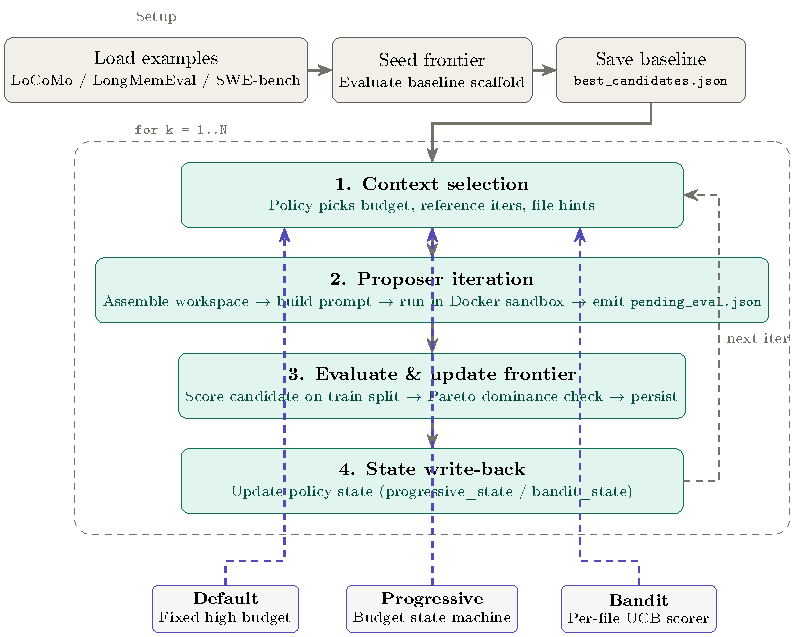
\includegraphics[width=\linewidth]{figures/system_overview.pdf}
  \vspace{-4pt}
  \caption{System overview. The setup phase evaluates baseline harnesses
  to seed the Pareto frontier. Each optimization iteration selects a
  context budget (via one of three policies), assembles a sandboxed
  workspace, runs the proposer, evaluates the candidate, and writes back
  policy state. The loop repeats for $N$ iterations.}
  \label{fig:system_overview}
\end{figure}

\subsection{Progressive Policy}
\label{sec:progressive}

The progressive policy implements a budget state machine
(Figure~\ref{fig:progressive_fsm}) that starts cheap and escalates
only when the optimization stalls. The hypothesis motivating this
design is that early breakthroughs are driven by focused, narrow
contexts; we defer empirical confirmation to
\S\ref{sec:experiments}.

\paragraph{State machine.}
Let $b_k$ denote the budget at iteration~$k$ and let
$\mathrm{improved}_k$ be the indicator that iteration~$k$ produced a new
entry on the Pareto frontier~$\mathcal{F}$. The transition rule is:
\begin{equation}
  b_{k+1} =
  \begin{cases}
    \texttt{low}    & \text{if } k < k_0 \text{ or } \mathrm{improved}_k, \\
    \texttt{medium} & \text{if } b_k = \texttt{low}
                      \text{ and } \neg\,\mathrm{improved}_k, \\
    \texttt{high}   & \text{if } b_k \in \{\texttt{medium},\texttt{high}\}
                      \text{ and } \neg\,\mathrm{improved}_k,
  \end{cases}
  \label{eq:progressive}
\end{equation}
where $k_0\!=\!5$ is a warm-up period during which the budget is forced
to \texttt{low}. The critical property is that any improvement
resets the budget to~\texttt{low}, so the system spends most iterations
at cheap, narrow context and only escalates to \texttt{high} after
consecutive stalls.

\paragraph{Prompt construction.}
Each tier exposes a different slice of the history
(Table~\ref{tab:budgets}): \texttt{low} surfaces a single best
iteration with the worst as anti-pattern; \texttt{medium} expands to
the top-3 by passrate; \texttt{high} feeds the full history and lets
the proposer infer roles from the cumulative iteration summary.

\begin{table}[h]
\centering
\small
\begin{tabular}{@{}lccc@{}}
\toprule
 & \texttt{low} & \texttt{medium} & \texttt{high} \\
\midrule
Reference iters & best\,1 + worst & best\,3 + worst & full history \\
Trace scope & last\,1 & last\,3 & all \\
\bottomrule
\end{tabular}
\vspace{2pt}
\caption{Reference-iteration exposure under the \emph{progressive}
budget tiers. ``Trace scope'' controls how many recent per-task
evaluation traces are included in each reference bundle. The bandit
policy uses a different per-budget selection
(\S\ref{sec:bandit}).}
\label{tab:budgets}
\end{table}

\begin{figure}[t]
  \centering
  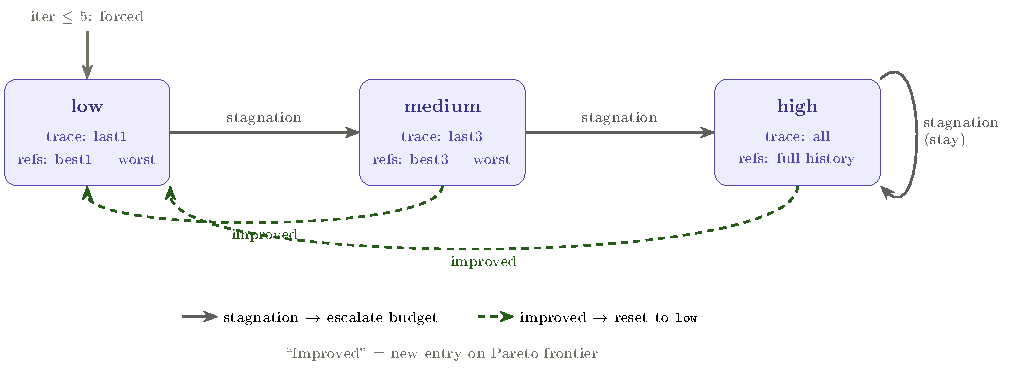
\includegraphics[width=0.92\linewidth]{figures/progressive_fsm.pdf}
  \vspace{-4pt}
  \caption{Progressive policy state machine. Solid arrows: budget
  escalation on stagnation (no new Pareto entry). Dashed arrows: reset
  to \texttt{low} on any improvement. The first $k_0\!=\!5$ iterations
  are forced to \texttt{low}.}
  \label{fig:progressive_fsm}
\end{figure}

\subsection{Bandit Policy}
\label{sec:bandit}

The bandit policy treats every readable file in the workspace as an arm
of a multi-armed bandit (Figure~\ref{fig:bandit_flow}) and uses
per-file utility estimates to construct a hot workspace that
concentrates the proposer's attention on files whose past reads
correlated with positive outcomes.

\paragraph{Reward signal.}
At the end of iteration~$k$, the harness computes a rolling $z$-score
reward from the candidate's passrate:
\begin{equation}
  r_k =
  \begin{cases}
    -\gamma/4 & \text{if no valid candidate was produced,} \\[2pt]
    \operatorname{clip}\!\bigl(
      (p_k - \hat\mu_k) \,/\, \hat\sigma_k,\;\pm\gamma
    \bigr) & \text{otherwise,}
  \end{cases}
  \label{eq:reward}
\end{equation}
where $p_k\!=\!p(h_k)$, and $\hat\mu_k,\hat\sigma_k$ are the mean and
standard deviation of passrates over the most recent~$W\!=\!8$
iterations (with $\hat\sigma_k \ge \sigma_{\min}$). The clip bound is
$\gamma\!=\!2$, and an iteration counts as a success when
$r_k > 0$. The fixed penalty $-\gamma/4 = -0.5$ for invalid candidates
is large enough to discourage repeated failure modes but smaller in
magnitude than the worst-case clipped negative reward, so a single
crash does not dominate downstream utility estimates. Normalizing
against the recent window---rather than the global best---lets a
meaningful rebound during a stagnation stretch still earn positive
reward.

\paragraph{Per-file utility.}
After computing the reward, the harness records which files the proposer
read, wrote, and changed. For each file~$f$ in the discretionary read
pool (excluding a fixed set of always-included core files), the
policy score combines four components:
\begin{equation}
  S_f = \underbrace{0.7\,\Delta_f^{\text{bin}}
        + 0.3\,\Delta_f^{\text{rew}}}_{\text{utility}}
        - \underbrace{\lambda\,\log\!\bigl(1 + \bar\ell_f / L\bigr)}_{\text{cost}}
        + \underbrace{c\,\sqrt{\frac{\ln(k+1)}{n_f+1}}}_{\text{UCB bonus}},
  \label{eq:policy_score}
\end{equation}
where $\Delta_f^{\text{bin}}$ is file~$f$'s binary success rate
relative to the global success rate, smoothed by a
Beta($\alpha,\alpha$) prior; $\Delta_f^{\text{rew}}$ is file~$f$'s
mean reward relative to the global mean, smoothed by $\alpha$
pseudo-observations at the global mean ($\alpha\!=\!2$);
$\bar\ell_f$ is the average number of lines read from~$f$, $n_f$ is
the read count, and $L\!=\!500$ is a line-count normalizer. The UCB
bonus ($c\!=\!0.15$) ensures under-explored files are sampled before
their utility is written off, and the cost term ($\lambda\!=\!0.05$)
discourages over-reading large files.

\paragraph{Hot workspace and budget.}
Files are sorted by $S_f$; a fixed set of core files (target
scaffold source, base classes, summary files) is pinned, the top-8
scored files join the hot list (800-line read cap) and the
next-12 form the warm list (300-line cap). Together they constitute
the hot workspace surfaced to the proposer as advisory hints; other
files remain readable on demand. The budget tier is
\begin{equation}
  b_k =
  \begin{cases}
    \texttt{low}    & \text{if } k\!\le\!1 \text{ or no file stats,} \\
    \texttt{high}   & \text{if stagnation} \ge \theta\!=\!4, \\
    \texttt{medium} & \text{otherwise.}
  \end{cases}
  \label{eq:bandit_budget}
\end{equation}
Unlike the progressive policy, the bandit has no monotonic escalation
path: it stays at \texttt{medium} indefinitely as long as improvements
arrive before the stagnation window closes. At \texttt{high} budget
all prior iterations are referenced; at \texttt{medium} the bandit
selects up to five (iterations where hot files appeared, the top-3 by
passrate, and the last improving iteration); at \texttt{low} no raw
references are provided.

\begin{figure}[t]
  \centering
  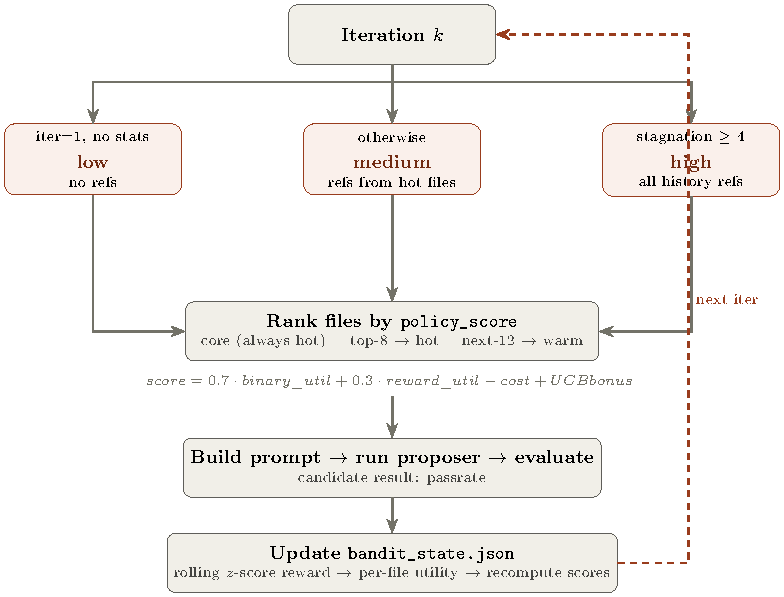
\includegraphics[width=0.88\linewidth]{figures/bandit_flow.pdf}
  \vspace{-4pt}
  \caption{Bandit policy decision flow. Each iteration starts with a
  budget decision based on stagnation count, ranks files by
  $S_f$~(Eq.~\ref{eq:policy_score}), runs the proposer, then feeds the
  reward (Eq.~\ref{eq:reward}) back to update per-file utility
  estimates.}
  \label{fig:bandit_flow}
\end{figure}

\subsection{Default Policy}
\label{sec:default}

The default policy is the fixed-context baseline that all prior
harness-optimization systems implicitly adopt: every iteration uses
\texttt{high} budget with no role labels, so the proposer sees the
full file tree and complete history. We retain it as a controlled
baseline to isolate the contribution of adaptive iteration- and
file-level context selection.

\subsection{Benchmark Integration}
\label{sec:benchmarks}

The shared loop and policy logic are identical across tasks; only the
evaluation function~$\operatorname{eval}(\cdot)$ and the editable
source set in~$W_k$ are specialized per benchmark. We evaluate on
LoCoMo (conversational-memory QA, scored by token-F1 against a
reference answer)~\cite{maharana2024locomo}, LongMemEval (long-term
memory, also token-F1)~\cite{wu2024longmemeval}, and SWE-bench
Verified (software engineering, scored by patch-pass against the
hidden test suite)~\cite{jimenez2024swebench}, spanning both
memory-retrieval and coding-agent harnesses.
